\chapter{Introduction}


\section{Data}

\begin{description}
    \item[Data] \marginnote{Data}
        Collection of raw values.

    \item[Information] \marginnote{Information}
        Organized data (e.g. relationships, context, \dots).

    \item[Knowledge] \marginnote{Knowledge}
        Understanding information.
\end{description}


\subsection{Data sources}
\begin{description}
    \item[Transaction] \marginnote{Transaction}
        Business event that generates or modifies data in an information system (e.g. database).

    \item[Signal] \marginnote{Signal}
        Measure produced by a sensor.

    \item[External subjects]
\end{description}


\subsection{Software}
\begin{description}
    \item[\Ac{oltp}] \marginnote{\Acl{oltp}} 
        Class of programs to support transaction-oriented applications and data storage.
        Suitable for real-time applications.

    \item[\Ac{erp}] \marginnote{\Acl{erp}} 
        Integrated system to manage all the processes of a business.
        Uses a shared database for all applications.
        Suitable for real-time applications.
\end{description}


\subsection{Insight}
Decisions can be classified as:
\begin{descriptionlist}
    \item[Structured] \marginnote{Structured decision}
        Established and well-understood situations.
        What is needed is known.
    \item[Unstructured] \marginnote{Unstructured decision}
        Unplanned and unclear situations.
        What is needed for the decision is unknown.
\end{descriptionlist}

Different levels of insight can be extracted by:
\begin{descriptionlist}
    \item[\Ac{mis}] \marginnote{\Acl{mis}}
        Standardized reporting system built on an existing \ac{oltp}.
        Used for structured decisions.

    \item[\Ac{dss}] \marginnote{\Acl{dss}}
        Analytical system to provide support for unstructured decisions.

    \item[\Ac{eis}] \marginnote{\Acl{eis}}
        Formulate high-level decisions that impact the organization.

    \item[\Ac{olap}] \marginnote{\Acl{olap}}
        Grouped analysis of multidimensional data.
        Involves a large amount of data.

    \item[\Ac{bi}] \marginnote{\Acl{bi}}
        Applications, infrastructure, tools and best practices to analyze information.
\end{descriptionlist}



\begin{description}
    \item[Big data] \marginnote{Big data}
        Large and/or complex and/or fast-changing collection of data that traditional DBMSs are unable to process.
        \begin{description}
            \item[Structured] e.g. relational tables.
            \item[Unstructured] e.g. videos.
            \item[Semi-structured] e.g. JSON.   
        \end{description}

    \item[Anaylitics] \marginnote{Anaylitics}
        Structured decision driven by data.

    \item[Data mining] \marginnote{Data mining}
        Discovery process for unstructured decisions.
        \begin{figure}[ht]
            \centering
            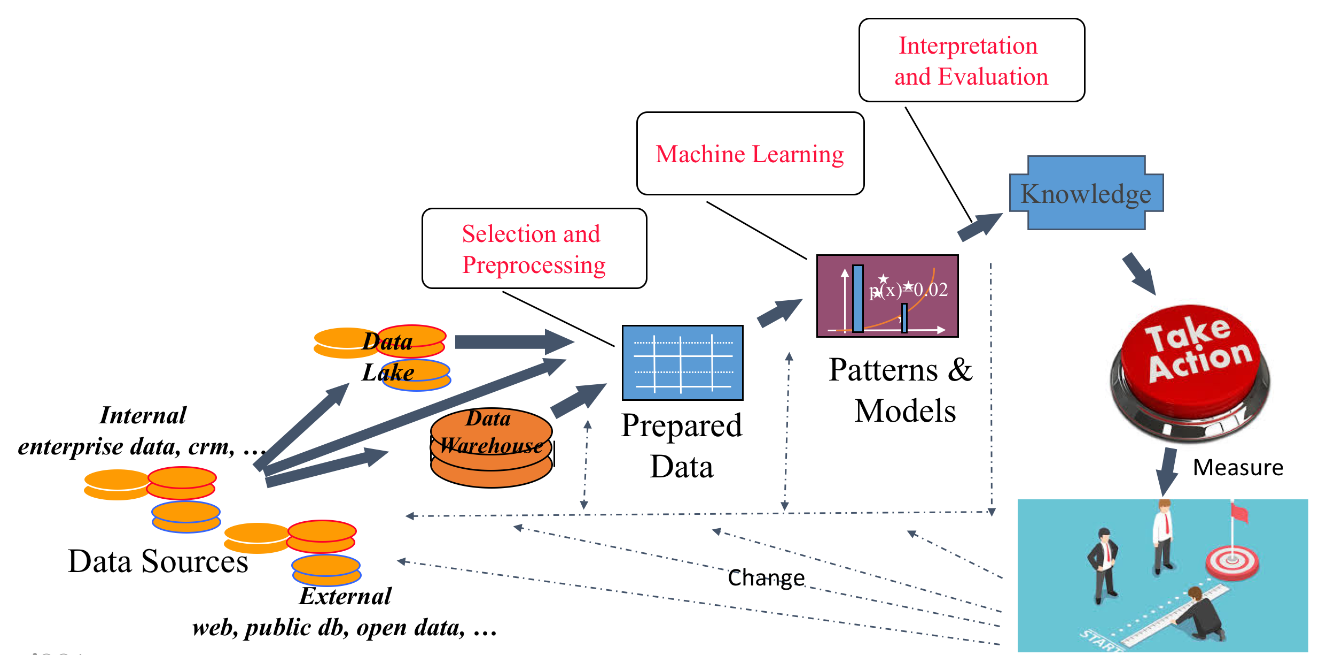
\includegraphics[width=0.8\textwidth]{img/data_mining_process.png}
            \caption{Data mining process}
        \end{figure}

    \item[Machine learning] \marginnote{Machine learning}
        Learning models and algorithms that allow to extract patterns from data.
\end{description}